\documentclass[11pt,a4paper, dvipdfmx]{jsarticle}
\usepackage{amsmath,amssymb}
\usepackage{amsthm}
\usepackage{ascmac}
\usepackage{bm}
\usepackage[dvipdfmx]{graphicx}	% required for `\includegraphics' (yatex added)
\usepackage{setspace}           % required for `\doublespace'
\usepackage{tikz}
\usepackage{tikz-cd}
\usetikzlibrary{angles, positioning, shapes, arrows.meta, decorations.pathmorphing}
%\usetikzlibrary{intersections, calc, arrows, positioning, arrows.meta}
\usepackage{tcolorbox}  % 定理環境の装飾
\tcbuselibrary{skins, breakable, theorems}
\usepackage{xcolor}
\usepackage{natbib}
\usepackage{pxrubrica}
\usepackage[margin=30truemm, left=40truemm, right=40truemm]{geometry}
\usepackage{thmbox}     % required for theorem environment with side bar
%
\setlength{\parskip}{3mm} %段落間にスペースを入れる


% \pagestyle{myheadings}
% \markright{\footnotesize \sf 2022秋期「哲学者のための数学」授業資料(大塚淳) \ \ 配布禁止}


\theoremstyle{definition}
\newtheorem[S]{exercise}{練習問題}[section]
\newtheorem[S]{example}{事例}[section]
\newtheorem[S]{fact}{事実}[section]
\newtheorem[S]{attn}{注意}[section]
\newtheorem[S]{develop}{発展}[section]
\renewcommand{\theattn}{}

\newtcbtheorem[auto counter, number within=section]{rei}{事例}{
    breakable,
    coltitle=black,
    fonttitle=\bfseries,
    enhanced, colback=white, frame hidden, borderline west = {0.5pt}{5pt}{black},
%    number freestyle={\noexpand\thesection.\noexpand\arabic{\tcbcounter}}
}{rei}

\newtcbtheorem[auto counter, number within=section]{prop}{命題}{
    breakable,
    coltitle=black,
    fonttitle=\bfseries,
    enhanced, colback=white, frame hidden, borderline west = {0.5pt}{5pt}{black},
%    number freestyle={\noexpand\thesection.\noexpand\arabic{\tcbcounter}}
}{prop}

\newtcbtheorem[number within=section]{renshu}{練習問題}{
    breakable,
    coltitle=black,
    fonttitle=\bfseries,
    enhanced, colback=white, frame hidden, borderline west = {0.5pt}{5pt}{black}
}{renshu}


\newtcbtheorem[number within=section]{hatten}{発展}{
    breakable,
    coltitle=black,
    fonttitle=\bfseries,
    enhanced, colback=white, frame hidden, borderline west = {0.5pt}{5pt}{black}
}{renshu}


\newtcbtheorem[number within=section]{dfn}{定義}{
    fonttitle=\bfseries,
    enhanced, colback=white
}{dfn}


% Bold face capital letters:
\newcommand{\bfzero}{\boldsymbol{0}}
\newcommand{\bfone}{\boldsymbol{1}}
\newcommand{\bfA}{\boldsymbol{A}}
\newcommand{\bfB}{\boldsymbol{B}}
\newcommand{\bfC}{\boldsymbol{C}}
\newcommand{\bfD}{\boldsymbol{D}}
\newcommand{\bfE}{\boldsymbol{E}}
\newcommand{\bfF}{\boldsymbol{F}}
\newcommand{\bfG}{\boldsymbol{G}}
\newcommand{\bfH}{\boldsymbol{H}}
\newcommand{\bfI}{\boldsymbol{I}}
\newcommand{\bfJ}{\boldsymbol{J}}
\newcommand{\bfK}{\boldsymbol{K}}
\newcommand{\bfL}{\boldsymbol{L}}
\newcommand{\bfM}{\boldsymbol{M}}
\newcommand{\bfN}{\boldsymbol{N}}
\newcommand{\bfO}{\boldsymbol{O}}
\newcommand{\bfP}{\boldsymbol{P}}
\newcommand{\bfQ}{\boldsymbol{Q}}
\newcommand{\bfR}{\boldsymbol{R}}
\newcommand{\bfS}{\boldsymbol{S}}
\newcommand{\bfT}{\boldsymbol{T}}
\newcommand{\bfU}{\boldsymbol{U}}
\newcommand{\bfV}{\boldsymbol{V}}
\newcommand{\bfW}{\boldsymbol{W}}
\newcommand{\bfX}{\boldsymbol{X}}
\newcommand{\bfY}{\boldsymbol{Y}}
\newcommand{\bfZ}{\boldsymbol{Z}}

\newcommand{\bfa}{\boldsymbol{a}}
\newcommand{\bfb}{\boldsymbol{b}}
\newcommand{\bfc}{\boldsymbol{c}}
\newcommand{\bfd}{\boldsymbol{d}}
\newcommand{\bfe}{\boldsymbol{e}}
\newcommand{\bff}{\boldsymbol{f}}
\newcommand{\bfk}{\boldsymbol{k}}
\newcommand{\bfm}{\boldsymbol{m}}
\newcommand{\bfn}{\boldsymbol{n}}
\newcommand{\bfo}{\boldsymbol{o}}
\newcommand{\bfp}{\boldsymbol{p}}
\newcommand{\bfq}{\boldsymbol{q}}
\newcommand{\bfr}{\boldsymbol{r}}
\newcommand{\bfs}{\boldsymbol{s}}
\newcommand{\bft}{\boldsymbol{t}}
\newcommand{\bfu}{\boldsymbol{u}}
\newcommand{\bfv}{\boldsymbol{v}}
\newcommand{\bfw}{\boldsymbol{w}}
\newcommand{\bfx}{\boldsymbol{x}}
\newcommand{\bfy}{\boldsymbol{y}}
\newcommand{\bfz}{\boldsymbol{z}}



% BB (???) capital letters:
\newcommand{\bbA}{\mathbb{A}}
\newcommand{\bbB}{\mathbb{B}}
\newcommand{\bbC}{\mathbb{C}}
\newcommand{\bbD}{\mathbb{D}}
\newcommand{\bbE}{\mathbb{E}}
\newcommand{\bbF}{\mathbb{F}}
\newcommand{\bbG}{\mathbb{G}}
\newcommand{\bbI}{\mathbb{I}}
\newcommand{\bbN}{\mathbb{N}}
\newcommand{\bbP}{\mathbb{P}}
\newcommand{\bbQ}{\mathbb{Q}}
\newcommand{\bbR}{\mathbb{R}}
\newcommand{\bbU}{\mathbb{U}}
\newcommand{\bbV}{\mathbb{V}}
\newcommand{\bbX}{\mathbb{X}}
\newcommand{\bbY}{\mathbb{Y}}
\newcommand{\bbZ}{\mathbb{Z}}
\newcommand{\bbone}{{\ifmmode\mathrm{1\!l}\else\mbox{\(\mathrm{1\!l}\)}\fi}}


% Caligraphic math capital letters:
\newcommand{\mcalA}{\mathcal{A}}
\newcommand{\mcalB}{\mathcal{B}}
\newcommand{\mcalC}{\mathcal{C}}
\newcommand{\mcalD}{\mathcal{D}}
\newcommand{\mcalE}{\mathcal{E}}
\newcommand{\mcalF}{\mathcal{F}}
\newcommand{\mcalG}{\mathcal{G}}
\newcommand{\mcalH}{\mathcal{H}}
\newcommand{\mcalI}{\mathcal{I}}
\newcommand{\mcalJ}{\mathcal{J}}
\newcommand{\mcalK}{\mathcal{K}}
\newcommand{\mcalL}{\mathcal{L}}
\newcommand{\mcalM}{\mathcal{M}}
\newcommand{\mcalN}{\mathcal{N}}
\newcommand{\mcalO}{\mathcal{O}}
\newcommand{\mcalP}{\mathcal{P}}
\newcommand{\mcalQ}{\mathcal{Q}}
\newcommand{\mcalS}{\mathcal{S}}
\newcommand{\mcalT}{\mathcal{T}}
\newcommand{\mcalU}{\mathcal{U}}
\newcommand{\mcalV}{\mathcal{V}}
\newcommand{\mcalX}{\mathcal{X}}
\newcommand{\mcalY}{\mathcal{Y}}
\newcommand{\mcalZ}{\mathcal{Z}}

% Graph nodes notations:
\newcommand{\PA}{\mathit{PA}}
\newcommand{\bfPA}{\mathbf{PA}}
\newcommand{\CH}{\mathit{CH}}
\newcommand{\bfCH}{\mathbf{CH}}
\newcommand{\DS}{\mathit{DS}}
\newcommand{\bfDS}{\mathbf{DS}}
\newcommand{\ND}{\mathit{ND}}
\newcommand{\bfND}{\mathbf{ND}}
\newcommand{\AN}{\mathit{an}}
\newcommand{\bfAN}{\mathbf{an}}
\newcommand{\pa}{\mathit{pa}}
\newcommand{\bfpa}{\mathbf{pa}}
\newcommand{\ch}{\mathit{ch}}
\newcommand{\bfch}{\mathbf{ch}}
\newcommand{\ds}{\mathit{ds}}
\newcommand{\bfds}{\mathbf{ds}}
\newcommand{\nd}{\mathit{nd}}
\newcommand{\bfnd}{\mathbf{nd}}
\newcommand{\an}{\mathit{an}}
\newcommand{\bfan}{\mathbf{an}}



\DeclareMathOperator*{\argmax}{arg\,max}
\DeclareMathOperator*{\argmin}{arg\,min}
\DeclareMathOperator*{\argsup}{arg\,sup}
\DeclareMathOperator*{\arginf}{arg\,inf}
\DeclareMathOperator{\erfc}{erfc}
\DeclareMathOperator{\diag}{diag}
\DeclareMathOperator{\cum}{cum}
\DeclareMathOperator{\sgn}{sgn}
\DeclareMathOperator{\tr}{tr}
\DeclareMathOperator{\spn}{span}
\DeclareMathOperator{\adj}{adj}
\DeclareMathOperator{\E}{\mathbb{E}}
\DeclareMathOperator{\var}{Var}
\DeclareMathOperator{\cov}{Cov}
\DeclareMathOperator{\corr}{corr}
\DeclareMathOperator{\sech}{sech}
\DeclareMathOperator{\sinc}{sinc}
\DeclareMathOperator*{\lms}{l.i.m.\,}
\newcommand{\varop}[1]{\var\left[{#1}\right]}
\newcommand{\covop}[2]{\cov\left({#1},{#2}\right)}
\newcommand{\T}{^\textrm{T}}
\newcommand\indep{\protect\mathpalette{\protect\independenT}{\perp}}
\def\independenT#1#2{\mathrel{\rlap{$#1#2$}\mkern2mu{#1#2}}}

\newcommand{\bfalpha}{\boldsymbol{\alpha}}
\newcommand{\bfbeta} {\boldsymbol{\beta}}
\newcommand{\bfgamma}{\boldsymbol{\gamma}}
\newcommand{\bfeta}  {\boldsymbol{\eta}}
\newcommand{\bftheta}{\boldsymbol{\theta}}
\newcommand{\bflambda}   {\boldsymbol{\lambda}}
\newcommand{\bfmu}   {\boldsymbol{\mu}}
\newcommand{\bfnu}   {\boldsymbol{\nu}}
\newcommand{\bfxi}   {\boldsymbol{\xi}}
\newcommand{\bfpsi}  {\boldsymbol{\psi}}
\newcommand{\bfphi}   {\boldsymbol{\phi}}
\newcommand{\bfrho}   {\boldsymbol{\rho}}
\newcommand{\bfvarepsilon}{\boldsymbol{\varepsilon}}
%\newcommand{\qed}{{qed}}
%\newcommand{\eqalignno}[1]{\begin{array}{ccccccc}#1\end{array}}

\newcommand{\bfGamma}{\boldsymbol{\Gamma}}
\newcommand{\bfTheta}{\boldsymbol{\Theta}}
\newcommand{\bfLambda}   {\boldsymbol{\Lambda}}
\newcommand{\bfPsi}  {\boldsymbol{\Psi}}
\newcommand{\bfPhi}   {\boldsymbol{\Phi}}
\newcommand{\bfSigma}  {\boldsymbol{\Sigma}}
\newcommand{\bfOmega}  {\boldsymbol{\Omega}}


% DISTRIBUTIOoNS: 
\newcommand{\normal}{\mathcal{N}}
\newcommand{\binomial}{\mathcal{B}}
\newcommand{\multinomial}{\mathcal{M}}
\newcommand{\exponential}{\mathcal{E}}
\newcommand{\geometric}{\mathcal{G}}
\newcommand{\poisson}{\mbox{Poisson}}
\newcommand{\uniform}{\mbox{Uniform}}

% Logic
\newcommand{\true}{\texttt{true}}
\newcommand{\false}{\texttt{false}}


%PSTricks (commande for latent nodes)
\newcommand{\lnode}[4]{ \cnode(#1){#2}{#3}\rput(#1){\footnotesize#4} }

% KEEPING TRACK OF WORK
\newcommand{\todo}[1]
{
{\color{red}{
[TODO: #1]}}
\addcontentsline{toc}{subsection}{TO DO: #1}
}

\newcommand{\fixme}[1]{{\color{red}{#1}}}

\newenvironment{answer}[1]
{\par \color{blue}{#1}}
{}


\newcommand{\note}[2]
{
{\color{red}{
[#1: #2]}}
}




\makeatletter
% define \citepos for posesive citation (e.g. Otsuka's (2015))
\DeclareRobustCommand\citepos
  {\begingroup
   \let\NAT@nmfmt\NAT@posfmt% ...except with a different name format
   \NAT@swafalse\let\NAT@ctype\z@\NAT@partrue
   \@ifstar{\NAT@fulltrue\NAT@citetp}{\NAT@fullfalse\NAT@citetp}}

\let\NAT@orig@nmfmt\NAT@nmfmt
\def\NAT@posfmt#1{\NAT@orig@nmfmt{#1's}}
\makeatother




% Code for drawing color circle used in topology (pathconnectedness)
\usepackage{xparse}
\ExplSyntaxOn

\keys_define:nn { colour_transition_circle } {
    inner   .fp_set:N   = \l__inner_radius,
    inner   .initial:n  = {2},
    outer   .fp_set:N   = \l__outer_radius,
    outer   .initial:n  = {3},
    angle   .fp_set:N   = \l__start_angle,
    angle   .initial:n  = {0}
}

\NewDocumentCommand \ColourTransitionCircle { O{} m } {
\group_begin:
    \keys_set:nn { colour_transition_circle } {#1}
    \clist_clear:N \l_tmpa_clist
    \clist_map_inline:nn {#2} {
        \clist_put_right:Nn \l_tmpa_clist {##1}
        %\clist_put_right:Nn \l_tmpa_clist {##1}
    }
    \exp_args:Nx \col_trans_circ:n \l_tmpa_clist
\group_end:
}

\cs_new_protected:Npn \col_trans_circ:n #1 {
    \int_step_inline:nnnn {1} {1} {\clist_count:n {#1} - 1} {
        \path[top~color=\clist_item:nn {#1} {##1}, bottom~color=\clist_item:nn {#1} {##1+1}, shading~angle={270-(180-360/\clist_count:n {#1})/2+(##1-1)*360/\clist_count:n {#1}+\fp_use:N \l__start_angle}] ({\fp_use:N \l__inner_radius*cos((##1-1)*360/\clist_count:n {#1}+\fp_use:N \l__start_angle)},{\fp_use:N \l__inner_radius*sin((##1-1)*360/\clist_count:n {#1}+\fp_use:N \l__start_angle)}) arc[radius = \fp_use:N \l__inner_radius, start~angle={(##1-1)*360/\clist_count:n {#1}+\fp_use:N \l__start_angle}, delta~angle=360/\clist_count:n {#1}] -- ({\fp_use:N \l__outer_radius*cos(##1*360/\clist_count:n {#1}+\fp_use:N \l__start_angle)},{\fp_use:N \l__outer_radius*sin(##1*360/\clist_count:n {#1}+\fp_use:N \l__start_angle)}) arc[radius = \fp_use:N \l__outer_radius, start~angle={##1*360/\clist_count:n {#1}+\fp_use:N \l__start_angle}, delta~angle=-360/\clist_count:n {#1}] -- cycle;
    }
    \path[top~color=\clist_item:nn {#1} {\clist_count:n {#1}}, bottom~color=\clist_item:nn {#1} {1}, shading~angle={180-180/\clist_count:n {#1}+\fp_use:N \l__start_angle}]({\fp_use:N \l__inner_radius*cos((\clist_count:n {#1}-1)*360/\clist_count:n {#1}+\fp_use:N \l__start_angle)},{\fp_use:N \l__inner_radius*sin((\clist_count:n {#1}-1)*360/\clist_count:n {#1}+\fp_use:N \l__start_angle)}) arc[radius = \fp_use:N \l__inner_radius, start~angle={(\clist_count:n {#1}-1)*360/\clist_count:n {#1}+\fp_use:N \l__start_angle}, delta~angle=360/\clist_count:n {#1}] -- ({\fp_use:N \l__outer_radius*cos(\clist_count:n {#1}*360/\clist_count:n {#1}+\fp_use:N \l__start_angle)},{\fp_use:N \l__outer_radius*sin(\clist_count:n {#1}*360/\clist_count:n {#1}+\fp_use:N \l__start_angle)}) arc[radius = \fp_use:N \l__outer_radius, start~angle={\clist_count:n {#1}*360/\clist_count:n {#1}+\fp_use:N \l__start_angle}, delta~angle=-360/\clist_count:n {#1}] -- cycle;
}

\ExplSyntaxOff
\usepackage{xcolor}

\begin{document}


\title{5. 位相}
\author{2025秋期「哲学者のための数学」授業資料(大塚淳)}
\date{ver. \today}
\maketitle

\section{位相とは何か・なぜそれを学ぶのか}

本章の主題は位相(topology)である.
大雑把にいうと,位相とは空間についての学問であり,近さや距離といったものを扱うための道具立てを与える.
我々が見てきた集合は,いわばそれぞれが独立した,つぶつぶの要素の集まりであって,その間の近さや距離みたいなものは考えられていなかった.
確かに空間や円・線などの幾何学的図形は点の集まりすなわち集合ではあるのだが,単なる集合には我々が「空間」に期待する様々な性質,例えば点と点の間の距離や近さといったものが備わっていない.
位相は,こうした幾何学的な性質を集合に与える.
その意味で,位相空間(位相が備わった集合)は,最もプリミティブで抽象的な意味での「空間」の概念だということができる\footnote{プリミティブ,というのは,例えば物理学などでおなじみの空間概念は,位相以外の条件をさらに必要とするからだ.具体的には,それらは多様体(manifold)といわれる,のであるが,本講では扱わない.}.

このようなことから,位相は空間や時間等を扱う物理学を始めとした自然科学において非常に重要な役割を持っている一方,哲学においては,それほど重視されてこなかった \citep{Mormann2020-ly, Fletcher2022-ve}.
しかしながら,空間や近さという概念は,哲学においても頻出の重要概念である.
多くの場合,そうした議論では暗にユークリッド空間がイメージされることが多いが,ユークリッド空間というのは多種多様な空間概念のうちのたった一つの特殊例にすぎないので,そのイメージに引きづられると物事の理解を歪めてしまうかもしれない.
それを防ぐためにも,位相一般についての知識を持っていることは望ましい.

位相を考えるには,二つのアプローチがある.
一つは,集合上に距離を導入して,距離空間(距離が定められた集合)の上で位相的性質を定めていく方法.
もう一つは,集合上のそれぞれの点の間の類似性を示すグルーピング(これを「開集合」と呼ぶ)を与えて,そこから距離を導く方法.
これらはトンネルを右から掘るか左から掘るかの違いのようなもので,最終的には同じことである.
本講義では,まず直感的でイメージしやすい前者から入り,その後でより抽象的な後者のアプローチへと進んでいくことにしよう.


\section{距離空間}
「空間」と呼ばれるものの最も基本的な特徴はなんだろうか.
イメージは人によって異なるかもしれないが,それぞれの地点が「距離」というものによって隔てられている,ということは空間の顕著な特徴だといえそうである.
数学的には,集合$S$の要素を地点と捉えれば,任意の2地点の間の距離は,非負実数への関数$d:S \times S \to \bbR^+_0$によって表すことができるだろう.
しかしこれを「距離」というからには,どんな関数でも良いわけではなく,我々が通常距離に期待している性質を満たしていてほしい.
それを定めるのが,以下の条件である.

\begin{dfn}{距離空間}{distance}
  集合$S$上に,次の条件を満たす\emph{距離関数}(distance function) $d:S \times S \to \bbR^+_0$ が定義されているとき,組$(S, d)$を距離空間と呼ぶ.
  \begin{enumerate}
    \item (正定値性)任意の$x,y \in S$について,$d(x, y) \geq 0$であり,かつ$d(x, y) = 0 \iff x=y$;
    \item (対称性)任意の$x,y \in S$について,$d(x, y) = d(y, x)$;
    \item (三角不等式)任意の$x, y, z \in S$について,$d(x, z) \leq d(x,y) + d(y,z)$.
  \end{enumerate}
\end{dfn}

正定値性条件(1)は,同じ時点間の距離はゼロであること,またもし2点間の距離がゼロならそれらは同じ点であることを述べている.
対称性(2)は,点$x$から$y$への「行き」の距離は,点$y$から$x$への「帰り」の距離と同じであることを述べている.
三角不等式(3)は,ある点$x$から別の点$z$まで行くときに,途中寄り道$y$することで距離が短くなることはない,ということを述べている.
これらは確かに,我々が「距離」というものについて持っている直観を表していそうだ.

\begin{rei}{ユークリッド空間}{Euclid}
  2次元座標$X \times Y$において,2点$a = (a_x, a_y), b=(b_x, b_y)$の間の距離を
  \[ d(a, b) = \sqrt{(a_x - b_x)^2 + (a_y - b_y)^2}\]
  と定めると,この$d$は距離となる.これは平面上のユークリッド距離といわれる.
  またこれを$n$次元に拡張した
  \[ d(a, b) = \sqrt{\sum_i^n(a_i - b_i)^2}\]
  も同様に距離となる.このような距離が入った空間を$n$次元ユークリッド空間と呼ぶ.
\end{rei}


\begin{rei}{類似性}{similarity}
類似性は,哲学において極めて重要な概念である.
ウィトゲンシュタインは『哲学探究』において,概念は必要十分条件によってカチッと定まるのではなく,単に家族のように互いに類似したものの緩い集まりに過ぎないと主張した(家族的類似性).
またデイヴィッド・ルイスによる反事実条件文や因果命題の分析では,可能世界の間の類似性/近さという概念が中心的な役割をなす.
こうした(非)類似性は,事物間の「距離」としてモデル化できる.
いま,類似性を測りたい事物の集合$X$として,その各元が持つ性質を,$X$から実数$\bbR$への関数$p_1, p_2, \dots, p_n:X \to \bbR$によって記述するとしよう.
例えば$X$を人の集合とし,$p_1$を各人の身長とすると,$p_1(a)$は$a$さんの身長である.
すると各人$a \in X$は,$(p_1(a), p_2(a), \dots, p_n(a))$という$n$次元空間上の一点(ベクトル)で表されることになる.
この空間を特徴空間と呼ぶ.
特徴空間上には上で見たユークリッド距離:
  \[ d_{\text{sim}}(a, b) = \sqrt{\sum_i^n(p_i(a) - p_i(b))^2}\]
が定義できる.
これは$a$さんと$b$さんが性質$p_1, p_2, \dots, p_n$の値においてどれだけ離れているかの指標になっている.
よってこの距離$d_{\text{sim}}$が小さいほど,二人は似ているということができる.

こうした類似性基準は,認知科学における概念のプロトタイプ説(概念を相互に類似した対象のクラスターと考える),自然言語処理における単語の分散表現(単語の意味を文脈の類似度から測る)など,非常に幅広く用いられている(ただしそこで用いられている距離は必ずしもユークリッド距離とは限らず,他の距離関数が用いられることもある).
\end{rei}

ユークリッド距離以外にも,様々な距離,すなわち定義\ref{dfn:distance}で見た正定値性・対称性・三角不等式を満たす関数が考えられる.
例えばユークリッド距離では差の二乗を用いたが,これを絶対値に置き換えたもの $d_M(a,b) = \sum_i^n|a_i - b_i|$は,マンハッタン距離と呼ばれる.
また自然言語処理では,2つの単語ベクトルがなす角度$\theta$によって類似度を測るコサイン類似度$cos\theta$が一般的である(図\ref{fig:distances}).
よって距離や類似性を考えるときは,どのような距離空間/関数を考えるのか,またそれが対象のモデリングにとって適切なのかどうかをよく考える必要がある.

\begin{figure}[h]
  \centering
  \begin{minipage}[b]{0.31\linewidth}
    \centering
    \begin{tikzpicture}
    \draw [-stealth](0,0)--(3,0) node [below right]{$x$};
    \draw [-stealth](0,0)--(0,3) node [above left]{$y$};
    
    \coordinate[label=above:a](a)at(.5,2.3);%点Aの定義
    \coordinate[label=right:b](b)at(2.4,.8);%点Bの定義
    \foreach\P in{a,b}\fill[black](\P)circle(0.06);
    \draw [color=red](a)--(b);
    \end{tikzpicture}
  \end{minipage}
  \begin{minipage}[b]{0.31\linewidth}
    \centering
    \begin{tikzpicture}
    \draw [-stealth](0,0)--(3,0) node [below right]{$x$};
    \draw [-stealth](0,0)--(0,3) node [above left]{$y$};
    
    \coordinate[label=above:a](a)at(.5,2.3);%点Aの定義
    \coordinate[label=right:b](b)at(2.4,.8);%点Bの定義
    \foreach\P in{a,b}\fill[black](\P)circle(0.06);
    \draw [color=red](a)--(2.4,2.3)--(b);
    \end{tikzpicture}
  \end{minipage}
  \begin{minipage}[b]{0.31\linewidth}
    \centering
    \begin{tikzpicture}
    \draw [-stealth](0,0)--(3,0) node [below right]{$x$};
    \draw [-stealth](0,0)--(0,3) node [above left]{$y$};
    
    \coordinate(o)at(0,0);%点Aの定義
    \coordinate[label=above:a](a)at(.5,2.3);%点Aの定義
    \coordinate[label=right:b](b)at(2.4,.8);%点Bの定義
    \foreach\P in{a,b}\fill[black](\P)circle(0.06);
    \draw [color=black](a)--(o)--(b);
    \draw pic[color=red, "$\theta$", draw, <->, angle eccentricity=1.2,angle radius=.8cm] {angle=b--o--a};%
    \end{tikzpicture}
  \end{minipage}
  \caption{様々な距離関数.(左)ユークリッド距離は,2点$(a,b)$を結ぶ直線の長さである.(中)マンハッタン距離は,2点間の$x$座標,$y$座標の違いを足したものになる(マンハッタンの街のように碁盤の目状に敷かれた道を移動している感覚.京都距離と呼んでも良いかも?).(右)コサイン距離は,2つの点がなすベクトルの間の角度のコサイン$\cos\theta$をとったもの.長さは関係なく,角度の開きだけが効いてくる.}
  \label{fig:distances}
\end{figure}

\begin{renshu}{}{}
座標軸上に一点をとり(上の点$a$でも良い),そこから(1)ユークリッド距離,(2)マンハッタン距離,(3)コサイン距離が等しい点の集合をそれぞれ座標上に書き入れよ.
\end{renshu}

% \begin{rei}{モード}{modes}
% ピアノの鍵盤には,「任意のキーから別のキー移動するステップの数」という距離が入っている.
% 例えば$C$と$F$の間の距離は,$C \to C^\# \to D \to D^\# \to E \to F$なのでと5ステップである.
% \end{rei}


\begin{rei}{世界の類似性}{possible_worlds}
$W$を可能世界の集合,$P = \{p_1, p_2, \dots, p_n\}$を命題の集合とする.
世界$w \in W$で命題$p_i$が成立していることを$p_i(w)=1$,成立していないことを$p_i(w)=0$で表すと,各世界は$n$次元の$0-1$空間内の点によって表現される(ちなみにこの空間は束になる).
これは$n$次元ユークリッド空間を$0$と$1$に制限しただけなので,事例\ref{rei:similarity}と同様にユークリッド距離が定義できる(ちなみに同様の仕方でマンハッタン距離も定義できる).
この距離は,2つの可能世界$w, w'$が命題$P$の枠内でどれだけ一致するかを測っている.
もし両者があらゆる命題$p_i$の真理値において一致するならば,$p_i(w) - p_i(w')=0$となり距離はゼロになる.
この場合,2つの可能世界$w, w'$は同じであると考える.
対称性と三角不等式は,ユークリッド距離の性質から満たされる.
\end{rei}
\begin{table}[htbp]
 \caption{可能世界$w_1, \dots, w_4$とそこでどの命題$p_1, \dots, p_4$が成立するかを表す表の例.例えば世界$w_1$では$p_1, p_2, p_4$が成立し,$p_3$が成立していない.}
 \centering
 \begin{tabular}[tb]{ccccc}
      & $p_1$ & $p_2$ & $p_3$ & $p_4$ \\ \hline
$w_1$ &  1  &  1  &  0  &  1  \\
$w_2$ &  0  &  0  &  1  &  1  \\
$w_3$ &  0  &  1  &  0  &  0  \\
$w_4$ &  1  &  0  &  0  &  1  
 \end{tabular}
 \label{tb:possible_worlds}
\end{table}

\begin{renshu}{}{}
 上の表\ref{tb:possible_worlds}に従い各世界間のユークリッド距離を計算し,それが距離関数の公理を満たしていることを確認せよ.
\end{renshu}

\section{開集合と閉集合}
上で見てきた距離は,集合$S$上の点の間の関係性を規定するものだった.
これを用いることで,今度は$S$内の部分集合について,様々な性質や区分を考えることができるようになる.
具体的には,例えば部分集合の内部や境界,外部を考えたり,開集合・閉集合という区分を導入することが可能になる.
そしてこの区分は,距離に勝るとも劣らない重要な役割を,位相において果たすことになる.
色々な定義が矢継ぎ早に出てきて面食らうかもしれないが,イメージできればそこまで難しいものでもないので,気負わず頑張って欲しい.
まずは,それらすべての定義の「素」となる開球の概念を導入しよう.

\begin{dfn}{開球と閉球}{balls}
 $(S, d)$を距離空間とする.空間内の一点$a \in S$をとり,ゼロでない正の実数$\epsilon \in \bbR^+$をとる.
このとき,集合
\[
  \{ x \in S | d(a, x) < \epsilon \}
\]
を,$a$を中心とする半径$\epsilon$の\emph{開球}(open ball)といい,$B_\epsilon(a)$と書く.% また
% \[
%   \{ x \in S | d(a, x) \leq \epsilon \}
% \]
% を,$a$を中心とする半径$\epsilon$の\emph{閉球}(closed ball)という.
\end{dfn}
これらを球と呼ぶのは,三次元空間内ではこれらが$a$を中心にしたボール状の領域を定めるからだ.
$S$が二次元のときは円板,一次元のときは線分のようになり,そして四次元以上のときは高次元の超球体になる.

この開球を使うと,集合の「内部」「境界」「外部」といった概念を定義できるようになる.
\begin{dfn}{内部・外部・境界}{interior}
  距離空間$(S, d)$内の部分集合$A \subset S$をとる.
  \begin{itemize}
    \item $a \in A$が$A$の\emph{内点}であるとは,$A$にすっぽり収まる開球がその周りにとれる,つまりある$\epsilon > 0$があり$B_\epsilon(a) \subset A$となること.
    $A$の内点すべての集合を$A$の\emph{内部}(interior)といい,$A^\circ$で表す.
    \item 一方,$s \in S$が$A$の補集合$A^C$の内点であるとき,それを$A$の\emph{外点}という.
    $A$の外点すべての集合を$A$の\emph{外部}(exterior)といい,$A^e$で表す.
    \item $b \in S$が$A$の\emph{境界点}であるとは,その周りにどう開球をとっても$A$と$A^C$の両方にかかってしまうこと,つまりどんな$\epsilon > 0$をとっても,$B_\epsilon(a)$が$A$の点と$A^C$の点両方を含むこと.
    $A$の境界点すべての集合を$A$の\emph{境界}(boundary)といい,$\partial A$で表す.
    \item $A$の内点と境界をあわせたものを,$A$の\emph{閉包}(closure)といい,$\bar{A}$と書く.つまり$\bar{A} = A^\circ \cup \partial A$である.
  \end{itemize}
\end{dfn}

% これはただ字面を追うより,視覚的にイメージした方がわかりやすい.
% 図は集合$A$を表している.この集合の点$p, p'$をとると,半径$\epsilon$を十分小さくとることで$A$に含まれるような開円を取ることができる.
% 一方で点$q$では,どんなに小さく半径をとっても,$B_\epsilon(q)$の一部は$A$の外にはみ出してしまう.
% そうした点は,それ以上少しでも広げると$A$を超えるという意味で,$A$の境界線上にあるといえる.
% よって開集合とは,そうした境界線を含まないような集合であるといえる.

\begin{figure}[htbp]
 \begin{center}
  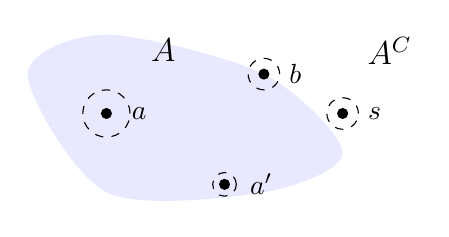
\begin{tikzpicture}
    \fill[blue!30, opacity=0.3] plot[smooth cycle] coordinates{(0,1) (1,1.5) (3,1)(4,0)(3,-.5)(1,-.5)};
   \node[left] (A) at (2, 1.3) {\large$A$};
   \node[left] (A) at (5, 1.3) {\large$A^C$};

   \fill (1,.5) circle (2pt);
   \draw[dashed] (1,.5) circle (0.3);
   \node[right] (a) at (1.2, .5) {$a$};

   \fill (2.5,-.4) circle (2pt);
   \draw[dashed] (2.5,-.4) circle (0.15);
   \node[right] (aa) at (2.7, -.4) {$a'$};

   \fill (3,1) circle (2pt);
   \draw[dashed] (3,1) circle (0.2);
   \node[right] (b) at (3.2, 1) {$b$};

   \fill (4,0.5) circle (2pt);
   \draw[dashed] (4,0.5) circle (0.2);
   \node[right] (s) at (4.2, 0.5) {$s$};
  \end{tikzpicture}
 \end{center}
 \caption{上図において,青い部分は集合$A$,白い部分はその補集合$A^C$を表す.$a, a'$の周りには$A$にすっぽり収まる開球をとれるため,内点になる.逆に外点$s$の周りには$A^C$に収まる開球が存在する.
 一方,境界上の$b$では,どんなに小さく$\epsilon$をとっても$B_\epsilon(b)$が$A$および$A^C$の双方にまたがってしまう.$A$はこうした境界を含まないとき開集合,すべて含むとき閉集合といわれる.
 一般に,開集合は破線,閉集合は実線で境界を描く.}
 \label{fig:openset}
\end{figure}

内点・外点・境界の区分は図\ref{fig:openset}を見れば一目瞭然だろう.
むしろ一目瞭然過ぎて,わざわざ様々な概念を持ち出してまで定義する意義があるのかと思うかもしれないが,このような定義によって,直感的に理解される「内部」「境界」などの概念が厳密に定まるのである.
そしてこれをもとに,位相において距離と並ぶもう一つの主役概念である,開集合と閉集合が以下のように定義される.

\begin{dfn}{開集合・閉集合}{open_closed}
  距離空間$(S, d)$内の部分集合$A \subset S$が\emph{開集合}(open set)であるとは,$A$のすべての点$a$がその内点であること,つまり$A = A^\circ$であること.

  一方$F \subset S$が\emph{閉集合}(closed set)であるとは,それが内点および境界点から構成されていること,つまり$F = \bar{F} = F^\circ \cup \partial F$であること.
\end{dfn}

つまり開集合は境界を含まず,閉集合は境界を含む.
ちなみに集合$F$が閉集合ならば,それを取り去った$F^C$には境界が含まれていないので開集合になる.逆に$F^C$が開集合なら,境界は$F$に含まれていなければならない.
ここから閉集合$F$は,「その補集合$F^C$が開集合であるような集合」とも定義できる.

開集合の典型例として,実数上の$a$より大きく$b$未満の開区間$(a, b) = \{x \in \bbR| a < x < b\}$があげられる.
確かに,この区間には端$a, b$が含まれていないが,端$a$にどんなに近い点$a'$を取ってきても,$\epsilon=|a-a'|/2$を半径とする$a'$中心の円をとれば,それが$a$より左側にはみ出ることはない.
一方,$a$以上$b$以下の閉区間$[a, b] = \{x \in \bbR| a \leq  x \leq  b\}$は閉集合である.
この場合,境界$a, b$を中心とする開円は明らかに$a$より左側ないし$b$より右側の部分とオーバーラップする.

ちなみにすべての集合が開集合か閉集合かのどちらかに区分されるわけでは\emph{ない}ことに注意しよう.
例えば,片方が開でもう片方が閉であるような区間$(a, b] := \{ x \in \bbR| a < x \leq b \}$は開集合でも閉集合でもない.
また開集合であり,かつ同時に閉集合であるような集合(\emph{clopen}と呼ばれる)もありえる.
全体集合$S$や空集合はその代表的存在だが,それ以外にも様々なものがある.

\begin{renshu}{}{}
  全体集合$S$および空集合が開かつ閉集合であることを示せ.
\end{renshu}


\begin{rei}{曖昧な概念}{open_concept}
  $A$を曖昧な概念,例えば「砂山」という概念の外延だとしてみよう.
  今,任意の砂山$a \in A$をとってきて,それとほんの数粒だけ砂の数が異なるものを考える.
  これはつまり$\epsilon > 0$について$B_\epsilon(a)$を考えるということだ.
  違いを十分少しにすれば,それらが突然砂山でなくなるということはないだろう.
  つまり$B_\epsilon(a) \subset A$となるような$\epsilon$があるだろう.
  よって曖昧な概念の外延は開集合であるといえる.
\end{rei}


\begin{rei}{意味の全体論}{semantic_holism}
クワインは有名な『経験主義の二つのドグマ』において,語の意味は一対一に対応する可能的経験によって定義されるのではなく,その語に関連する言語のネットワーク全体によって定まるのだという\emph{意味の全体論}(semantic holism)を提起した.
いま,全ての語のペアについてその(非)関連度が何らかの距離関数によって定まるとしよう.
例えば語「bachelor」は,「marriage 」「man」などと強く関連し,「life」などとは弱く関連し,「potato」などとはほとんど関係しない.
あるカットオフ$\epsilon$について,$B_\epsilon(w)$を語$w$の意味を定める関連語の集合と定める.
もちろん$\epsilon$は一意ではなく,様々な範囲で関連語を取ることによって,対象とする語$w$の意味の定まりかたは変わるだろう.
言語全体を$L$としよう.いかなる$w \in L$についても,その意味を定める関連語$B_\epsilon(w)$を当該言語の中でとることができる,つまりある$\epsilon$があり$B_\epsilon(w) \subset L$.
よって言語全体は開集合である.
これは全体論における「言語には縁がない」ことを表している.(吉井達也氏の考案)
\end{rei}

最後に,開集合と閉集合において成り立つ重要な性質について述べてこの節を閉じよう.
本来だったら証明しなければならないが,ここでは証明なしに事実として列挙する.気になる人は,手近な位相の教科書を参照してほしい.

\begin{prop}{開集合の性質}{open_set}
\begin{enumerate}
 \item $S$全体ならびに空集合$\emptyset$は開集合である.
 \item $O_1, O_2$が開集合ならば,$O_1 \cap O_2$は開集合.
 \item 任意の数(無限個でもよい)の開集合の族$\{ O_1, O_2, \dots \}$について,それら全体の和集合$\bigcup_i O_i$は開集合.
\end{enumerate}
\end{prop}

$S$自体が開集合なのは,どんな開球をとっても$S$から「はみ出す」ことはできないので当然だろう.
一方$\emptyset$については,そもそもいかなる点も含まないので,開集合の条件がトリビアルに満たされる.
2と3は開集合の共通部分と和がそれぞれ開集合であると言っているが,微妙に異なる.
和(3)に関しては,どれだけ,すなわち無限個の開集合の和をとっても開集合になる.
一方交わり(2)については,確かに$O_1 \cap O_2 \cap O_3 \dots$と共通部分をとっていったときにその結果は開集合になるのだが,しかしそれはあくまで有限個の範囲内であって,無限個の開集合の共通部分をとったとき,それが開集合になることは保証されない.
これは若干技巧的だが,次のような例を考えると分かる:
\[ A = \bigcap_{n=1}^{\infty} \bigg( -\frac{1}{n}, \frac{1}{n} \bigg) \]
右辺は,$(-1, 1) \cap (-1/2, 1/2) \cap \dots \cap (-1/n,1/n) \dots$という仕方で,どんどん小さくなる開区間を無限に考えたとき,その共通部分を抜き出せ,ということを言っている.
これは最終的に一点$A=\{0\}$に収束する.
しかし一点集合は開集合ではない,というのも0を中心とするいかなる開球$B_\epsilon(0)$も0以外を含んでしまうからだ.
以上から,無限個の開集合の共通部分は必ずしも開集合にならないことが示された.

同様に,閉集合については以下が成り立つ.

\begin{prop}{閉集合の性質}{closed_set}
  \begin{enumerate}
   \item $S$全体ならびに空集合$\emptyset$は閉集合である.
   \item $F_1, F_2$が閉集合ならば,$F_1 \cup F_2$は閉集合.
   \item 任意の数(無限個でもよい)の閉集合の族$\{ F_1, F_2, \dots \}$について,それら全体の共通部分$\bigcap_i F_i$は閉集合.
  \end{enumerate}
  \end{prop}
  つまり閉集合では開集合とは逆に,有限個の和と無限個の交わりについて閉じている.
  この意味でも,両者はちょうど対になるような存在だといえる.


% \begin{rei}{ウィトゲンシュタインと概念}{}  
% \end{rei}



\section{位相空間}

前節までは,距離空間をもとに開集合・閉集合などの位相的概念を導入し,その性質を導いた(実際の証明はしなかったが).
しかしその逆に,開集合・閉集合を命題\ref{prop:open_set}, \ref{prop:closed_set}で見たような性質をもつ集合族として天下り式に定めることで,位相空間を定義することもできる.
冒頭でも述べたように,このアプローチは若干抽象的でイメージがつかみにくい.
ではわざわざそれを入門的講義で扱うことの利点はどこにあるのか?
一つの理由として,距離関数というのはかなり「リッチ」な道具立てで,それを哲学的モデリングにおいて使いこなすのは中々難しい,という事情がある.
例えば現実世界と,京都が日本の首都であるような可能世界との間の距離がどれくらいか,正確に定める方法があるだろうか?
一方,開集合というのはある種「似た者同士」のグルーピングだと考えることがでる.
この「似たもののグルーピング」が,ものの「近さ」や「遠さ」の指標を構成する,ということが位相空間的アプローチの肝なのだが,哲学的なモデリングにとっては,こうしたグルーピングに基づくよりプリミティブな空間概念のほうが,使い勝手が良い場合が多いのである.

では早速,位相空間の定義を見てみよう.

\begin{dfn}{位相空間}{topology_open}
集合$T$の部分集合の族$\mcalO$が以下の条件を満たすとき,$\mcalO$は$T$の\emph{位相}であるという.
このとき$T$を(位相$\mcalO$を持つ)\emph{位相空間}といい,$(T, \mcalO)$で表す.
また$\mcalO$の要素である部分集合$O \subset T, O \in \mcalO$を開集合という.
\begin{enumerate}
 \item $\emptyset, T \in \mcalO$.
 \item $O_1, O_2 \in \mcalO$ならば$O_1 \cap O_2 \in \mcalO$.
 \item 任意の数(無限であっても良い)の$O_i \in \mcalO, i \in I$に対し,$\bigcup_{i \in I} O_i \in \mcalO$.
\end{enumerate}
\end{dfn}

これはちょうど,命題\ref{prop:open_set}で見た開集合の性質にほかならない.
ここでは逆に,有限個の交わりと無限個の和に対して閉じている集合の族として開集合を\emph{定義}している.
つまり,開集合をグルーピングとして捉えるという上の方針に従えば,二つのグループに対し「その共通部分」というグループが存在し,また無限個のグループに対し「それらどれかに含まれる」というグループが存在する,そのような仕方でグルーピングというものを考える,ということだ.

公理2と3の違い---有限個の交わりと無限個の和の違い---が効いてくるのは,$T$が無限集合であるときだけだ.
有限集合ではそもそも有限個の部分集合しかとれないので,$\mcalO$に含まれる任意の部分集合のペアについて,その合併と共通部分が再び$\mcalO$に含まれていれば,$(T, \mcalO)$は位相空間を構成する.
そしてその場合,位相の条件は4章で見た有限束の条件「任意の二元に関し結びと交わりが存在する」に一致する.
例えば$T:=\{a, b, c\}$とし,開集合として$\mcalO_1 := \{ \emptyset, \{a \}, \{b\}, \{a,b\}, \{a,b,c\} \}$をとってみよう.
この束構造は以下左のようになり,すべての結び・交わりが$\mcalO$に含まれているのでこれは位相を与える.
一方,$\mcalO_2 := \{ \emptyset, \{a \}, \{a,b\}, \{b,c\}, \{a,b,c\} \}$はそうではない.
これを開集合系にするためには,右図のように$\{b\} =  \{a,b\} \cap \{b,c\}$を含める必要がある.
\begin{figure}[h]
    \centering
    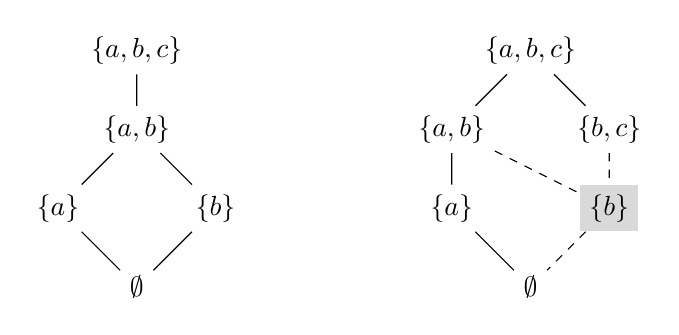
\begin{tikzpicture}
     \begin{scope}
      \node (abc)  at (1,3) {$  \{a, b, c\}$};
      \node (ab)  at (1,2) {$ \{a, b\} $};
      \node (a)  at (0,1) {$\{ a \}$};
      \node (b)  at (2,1) {$\{ b \}$};
      \node (0)  at (1,0) {$\emptyset$};
      \draw(abc)--(ab)--(a)--(0)--(b)--(ab);
     \end{scope}
     \begin{scope}[xshift=5cm]
      \node (abc)  at (1,3) {$ \{a, b, c\}$};
      \node (ab)  at (0,2) {$ \{a, b\} $};
      \node (bc)  at (2,2) {$ \{b, c\} $};
      \node (a)  at (0,1) {$\{ a \}$};
      \node[fill=gray!30] (b)  at (2,1) {$\{ b \}$};
      \node (0)  at (1,0) {$\emptyset$};
      \draw (bc)--(abc)--(ab)--(a)--(0);
      \draw[dashed] (bc)--(b)--(0);
      \draw[dashed] (ab)--(b);
     \end{scope}
    \end{tikzpicture}
    \caption{$T = \{a, b, c\}$としたときの開集合系の例$\mcalO_1$(左),$\mcalO_2$(右).}
    \label{fig:3bool} 
\end{figure}


\begin{renshu}{}{topologyex}
同様に$T:=\{a, b, c\}$としたとき
\begin{enumerate}
\item $\{ \emptyset, \{a,b\}, \{a,b,c\} \}$
\item $\{ \emptyset, \{a,b\}, \{c\}, \{a,b,c\} \}$
\item $\{ \emptyset, \{a\}, \{c\}, \{a,b,c\} \}$
\item $\{ \emptyset, \{a,b\}, \{a,c\}, \{a,b,c\} \}$
\item $\{ \emptyset, \{a\}, \{c\}, \{b, c\}, \{a,b,c\} \}$
\end{enumerate}
がそれぞれ$T$の位相となっているかどうか考えよ.またなっていない場合,最低限何を足したら位相となるかを答えよ.
\end{renshu}

位相空間はもととなる集合とその上の位相のペアとして定義される.
上の事例では同じ集合$T$を用いて異なる位相$(T, \mcalO_i)$が定義されることを見た.
一般に位相空間は,このように(集合, 位相)のペアとして指定する.
しかしいちいち位相を明示せずに,「$T$を位相空間とする」というようにいうこともある.
このような表現に出くわしたら,「集合$T$の上に,何か適当な位相$\mcalO$が乗っているんだな」と補って読んでほしい.


\begin{rei}{概念の外延の位相}{concept_topology}
$T$を地球上に存在する個物の集合とすると,それらに共通する\emph{性質}(property)を抜き出すことで個物を「似た者グループ」に分類することができるだろう.
例えば「赤い」という性質グループには,あなたの近所のポストや昨日食べたトマトが属する.
一方,「鉄製」というグループには,ポストは含まれるがトマトは入っていない.
このように様々な性質は異なった仕方で個物をグルーピングする.
こうして種々の性質の外延は,個物の集合$T$の部分集合である.
この部分集合としての性質が$T$に位相を定めるかどうかを見るためには,上述の3つの公理が満たされるかどうかをチェックしなければならない.
\begin{enumerate}
 \item まず「無」と「存在」という性質は,それぞれ$\emptyset$と$T$自体に対応する.
 \item 二つの性質があれば,両者に共通する性質も存在する.
 \item 複数の性質があれば,「そのうちどれか一つを性質をもつ」という性質が存在する.
\end{enumerate}
これらの公理が,我々の持っている性質観と一致するか,考えてみよう.
\end{rei}


位相空間に出くわしたら,それがちゃんと公理を満たしているかどうかを確認しよう.
特に,開集合族の(無限)和および(有限)共通部分がしっかりと位相に含まれているかどうかが重要である.
例えば上で,同じ性質を共有する事物を「似た者」としてグルーピングしたが,これが位相を構成するためには,複数の似た者グループ/開集合の和や共通部分もまたグループ/開集合となっているのでなければならない.
逆に,ある部分集合族が与えられたら,これらの部分集合の和や共通部分をすべて付け加えることで,位相を構成できる.
この作業を,「無限和と有限共通部分をとる」と表現することがある.

\begin{renshu}{}{}
 $T = \{$ アメリカ(A), 中国(C), 日本(J), メキシコ(M), イギリス(U) $\}$とする.
これらを何らかの基準で「似た者」とするグルーピングを考え,位相空間を構成せよ.当然この問題には答えはないが,それぞれのグループに説明があると望ましい.
\end{renshu}


\begin{rei}{可能世界}{possible_worlds2}
いま$W$を可能世界の集合とし,$P$を命題の集合としよう.
それぞれの命題$p \in P$について,その命題が成り立っている可能世界を集めたものを$W_p \subset W$と表し,「$p$世界($p$-worlds)」と呼ぶ.
つまり$W_p := \{ w \in W | p \text{ is true in } w \}$である.
このとき,部分集合族$\{ W_p \}_{p \in P}$が位相を構成する条件を定義\ref{dfn:topology_open}に照らして考えてみよう.
まず,条件1より,空集合と全体集合がなければならないが,$W_{\bot} = \emptyset, W_{\top}=W$より,矛盾$\bot$とトートロジー$\top$が$P$に含まれていなければならない.
次に$p, q \in P$について,
\begin{align*}
W_p \cap W_q &=  \{ w \in W | p \text{ is true in } w \} \cap \{ w \in W | q \text{ is true in } w \} \\
&= \{ w \in W | p \wedge q \text{ is true in } w \} \\
&= W_{p \wedge q}
\end{align*}
より,条件2を満たすためには$P$は有限個の$\wedge$について閉じている必要がある.
また同様に$P$が無限個の$\vee$についても閉じていれば,条件3が満たされ,可能世界の集合が位相を持つことになる.
この位相における開集合は各$p$世界であって,それは「命題$p$が成立している」という限りで「似ている」可能世界のグループを形成している.
\end{rei}

\begin{rei}{検証可能性}{}  
  今日を起点に,「$i$日目に観測されるカラスはすべて黒い」という命題を$p_i$で表す.
  当然,$p_0$は\emph{検証可能}(verifiable)だろう:今日カラスを観測して,それが黒いかどうかを確認すればよい.
  さらに,以下も成り立つと期待できる:
  \begin{itemize}
   \item $p_i$および$p_j$が検証可能ならば,$p_i \wedge p_j$($i$日目および$j$日目に観察されたカラスはすべて黒い)も検証可能.
   \item 任意の数の$i \in I$に対し,$p_i$が検証可能ならば,$\bigvee_i p_i$($I$日間のうちどれかの日に観測されたカラスはすべて黒い)も検証可能.
  \end{itemize}
  しかし「すべてのカラスが黒い」$\bigwedge_i p_i$という命題は検証可能ではない.
  上の事例で見たように,命題をそれが成立している可能世界の集合と同一視すると,この2つの要件は開集合の2,3に合致する.
  ここから,検証可能な命題は開集合であるといえる\citep{Kelly1996-hl,Genin2018-fr}.
  \end{rei}
  
\begin{renshu}{}{}
  表\ref{tb:possible_worlds}は,4つの命題$p_i, i = 1, 2, 3, 4$に対してそれぞれ$p_i$-世界を定めている.
  これらを含む最小限の位相空間$(W, \mcalO$)を構成せよ
  (ヒント:まず$\mcalO$には$W_{p_1} = \{w_1, w_4\}, W_{p_2} = \{w_1, w_3\}, W_{p_3} = \{w_2\}, W_{p_4} = \{w_1, w_2, w_4\}$が入っているので,これらを共通部分と合併で閉じればよい.)
 またそれぞれの開集合に対応する論理式を示せ.
\end{renshu}

ちなみに,定義\ref{dfn:topology_open}では開集合をベースに位相空間を定めたが,その代わりに閉集合を使って定義することも可能である.
3節で見たように,閉集合は開集合$O$の補集合$F = O^C$であり,開集合とはちょうど対となるような性質を持つのだった.
閉集合による位相の定義は,まず閉集合を\ref{prop:closed_set}で挙げたような性質を持つ集合の族$\mcalF$として定義していまい,そうした部分集合系を備えた集合として位相空間$(T, \mcalF)$を定める.
これは開集合による位相空間$(T, \mcalO)$の定義と同等であることが示せる.

% \begin{dfn}{閉集合系による位相の定義}{closed_topology}
%   集合$T$の部分集合の族$\mcalF$が以下の条件を満たすとき,$F \in \mcalF$を閉集合という.は$T$の\emph{位相}であるという.
%   このとき$T$を(位相$\mcalO$を持つ)\emph{位相空間}といい,$(T, \mcalO)$で表す.
%   また$\mcalO$の要素である部分集合$O \subset T, O \in \mcalO$を開集合という.
%   \begin{enumerate}
%     \item $\emptyset, T \in \mcalF$.
%     \item $F_1, F_2 \in \mcalF$ならば$F_1 \cup F_2 \in \mcalF$.
%     \item 任意の数(無限であっても良い)の$F_i \in \mcalF, i \in I$に対し,$\bigcap_{i \in I} F_i \in \mcalF$.
%   \end{enumerate}
% \end{dfn}


% \begin{example}
%  集合$T$に対して,その位相を冪集合$\mcalP(T)$で定める,つまり$\mcalO = \mcalP(T)$と定めることができる.
%  このとき,任意の部分集合$X \subset T$について,$X \in \mcalP(T)$かつ$X^c \in \mcalP(T)$であるので,$X$は開かつ閉(clopen)である.
% \end{example}

% \begin{example}
%  事例\ref{possibleworlds}で見た可能世界の位相において,任意の命題$a \in A$について$W_a \in \mcalO$としたとき,それぞれの$a$世界$W_a$はclopenだろうか.
% \end{example}


\section{さまざまな位相}
前節で見てきたように,同じ集合$T$に対して,異なる位相を入れることができる.
これは「何を似たものとするか」というグルーピングの仕方は一通りではなく,様々な仕方が考えられるということだ.

まず極端なケースとして,空集合と全体集合のみを開集合とする位相空間$\mcalO = \{\emptyset, T\}$が考えられる.
これを\emph{密着位相}(indiscrete topology)という.
密着位相は何も含まれないグループか,すべてを含むグループしか持たない.
だからここではすべての要素$x \in T$が一蓮托生に密着してしまっており,その中の一部だけを「似た者グループ」として取り出すことができない.

逆の極端ケースは,すべての部分集合を開集合とする位相空間$\mcalO = \mcalP(T)$である.
これを\emph{離散位相}(discrete topology)という.
ここでは,任意の部分集合が「似た者」グループを作る.
とりわけ,すべての要素$x \in T$は,それ自身が開集合$\{x\}$になっている.
なのですべての要素がより分けられてしまっていて,バラバラ(離散)になっている.

これを両端として,他にも様々な位相が考えられる.
ある位相$\mcalO_1$の開集合がすべて,別の位相$\mcalO_2$に含まれるとき,つまり$\mcalO_1 \subset \mcalO_2$のとき,$\mcalO_2$は$\mcalO_1$より\emph{細かい}(finer),$\mcalO_1$は$\mcalO_2$より\emph{粗い}(coarser)という.
$\mcalO_2$のほうが要素をより細かくグルーピングしている,というイメージだ.
この意味でいうと,密着位相は最も粗く,離散位相は最も細かい位相空間ということになる.
位相空間のモデリングでは,密着位相や離散位相はあまりおもしろくなく,対象に合わせた「ちょうどいい」細かさの位相を入れることがキモとなってくる.

\begin{renshu}{}{}
事例\ref{renshu:topologyex}でとりあげた集合 $T:=\{a, b, c\}$上の位相$\mcalO := \{ \emptyset, \{a \}, \{b\} \{a,b\}, \{a,b,c\} \}$について,(1) $\mcalO$より粗い位相,および(2)より細かい位相をそれぞれ一つづつ例示せよ.ただし密着位相と離散位相は除く.
\end{renshu}


\begin{renshu}{}{}
$T':=\{a, b, c, d\}$とする.
\begin{enumerate}
 \item 密着位相でも離散位相でもないような$T'$上の位相$\mcalO$を一つ例示せよ(ただし問2も参照せよ).
 \item 1よりも粗い位相/細かい位相をそれぞれ一つづつ例示せよ.ただし密着位相と離散位相は除く.
\end{enumerate}
\end{renshu}


\begin{hatten}{}{}
事例\ref{rei:possible_worlds2}で見たように,命題の集合$P$は可能世界に位相を定める.
いま,$P \subset P'$としたとき,それぞれの命題集合によって定められる可能世界の位相$\mcalO, \mcalO'$はどんな関係にあるだろうか.特に,$\mcalO'$は$\mcalO$より細かいだろうか.
\end{hatten}


% \begin{exercise}
% 有限集合$T$上の位相間の「より細かい」という関係は,どんな構造をなすだろうか.
% \end{exercise}




\section{連続写像}
次に,ある位相空間$X$から別の位相空間$Y$への写像を考えたい.
位相空間とは集合の上に位相である開集合族が乗っているだけなので,その集合上の写像$f:X \to Y$を位相空間$X$から$Y$への写像だと読み替えることができる.
ただしそうした写像は位相とはお構いなしに定義できるので,必ずしもそれらが$X$と$Y$の開集合を対応付けているとは限らない.
つまり,$X$の開集合$O_X$を$f$で送った像$f(O_X)$が$Y$の開集合である保証も,$Y$の開集合$O_Y$の逆像$f^{-1}(O_Y)$が$X$の開集合である保証もない.
前者の条件を満たす写像を特別に\emph{開写像}(open map),後者を満たす写像を\emph{連続写像}(continuous map)という.

\begin{dfn}{開写像と連続写像}{continous}
  $(X, \mcalO_X), (Y, \mcalO_Y)$をそれぞれ位相空間とし,$f:X \to Y$を写像とする.
  \begin{enumerate}
    \item $X$の任意の開集合$O_X \in \mcalO_X$に対し,$f$によるその像が$Y$の開集合である,つまり$f(O_X) \in \mcalO_Y$のとき,$f$を\emph{開写像}という.
    \item $Y$の任意の開集合$O_Y \in \mcalO_Y$に対し,$f$によるその逆像が$X$の開集合である,つまり$f^{-1}(O_Y) \in \mcalO_X$のとき,$f$を\emph{連続写像}という.
  \end{enumerate}  
\end{dfn}
  

開集合は「似た者同士」のグルーピングを与える,という本講のイメージに従えば,開写像は$X$でのグループが$Y$でもグループとして成立しているという意味で保存的な写像である.
一方,連続写像は$X$においてグループになっていないものは$Y$でグループにはならない,つまり写像$f$が$X$になかったグループを新たに作り出さない,という意味で保守的であるといえる.
この両者のうち,特に後者の連続写像は重要であり,位相空間における基本的な写像となっている.
そのため,以下でも連続写像に焦点をおいて考えてみよう.

\begin{rei}{アナロジー}{}
アナロジーとは,あるドメインから別のドメインへの,グルーピングを保存する写像として考えることができる.
例えば陸の動物の集合$X = \{lion, elephant, armadillo,...\}$から海の動物の集合$Y = \{shark, whale, turtle,...\}$への以下のような写像を考えよう:
\[
 f (lion) = shark, f(elephant)=whale, f(armadillo) = turtle,...
\]
一方$X, Y$には,各動物のグルーピング(捕食者,大きい等々)として開集合が定義されていると考える.
このとき,$Y$が$X$の良いアナロジーとなっているためには,$X$にもともと含まれないようなグループが$Y$にあってしまうと都合が悪い.
というのもその場合,任意の$Y$のグループを取り上げたとき,それが$X$について何か意味あることを表しているのかどうかがわからなくなってしまうからだ.
これはアナロジー写像$f$は連続であるべき,という要件にほかならない.
\end{rei}

写像はその定義域の位相が細かいほど,また値域の位相が粗いほど,連続になりやすくなる.
比喩的に言い換えれば,位相が細かいところから粗いところに流れる写像ほど,連続になりやすくなる.
極端な例としては,離散位相からの写像は値域に関わらずすべて連続であり,また密着位相への写像は定義域に関わらずすべて連続である(理由を考えてみよ).
このことを,$X$から$X$への恒等写像$i:X \to X$で考えてみよう.
これはすべての$x \in X$に対して$i(x) = x$となるような,「何もしない」写像である.
$X$上の異なる位相$\mcalO, \mcalO'$を考えると,$i$は位相空間$(X, \mcalO)$から$(X, \mcalO')$の写像だと考えることができる.
このとき
\[
 i \text{ が連続 } \iff \mcalO' \subset \mcalO
\]
が成り立つ.
というのも,$i$が連続であるとは,$\mcalO'$に含まれる任意の開集合$O'$について,$i^{-1}(O')=O'$自身が$\mcalO$に含まれる,ということにほかならないからだ.
つまり同一の集合上の位相空間を考えたとき,恒等写像の連続性は位相の細かさ/粗さに正確に対応している.


% 概念体系を別の概念体系に移す
% 連続写像の条件は?

「連続」というと,高校数学で習った実数関数の連続性を思い浮かべる人もいるかもしれない.
実のところその連続性は,ここで見た位相的な連続性にほかならない.
実数の集合$X$から$Y$への関数$f:X \to Y$を考える.
これが連続であるとは,$Y$の開区間$(a,b)$の逆像$f^{-1}(a,b)$が,$X$で開区間(ないしその無限和か有限共通部分)になっているということである.
例えば$f(x) = x^3-2x$では,$y$軸上の任意の開区間で曲線を$x$軸に投影すると,その影は開区間の和になっている.よってこの関数は連続である(図\ref{fig:realcontinuous}左).

\begin{figure}[h]
  \begin{minipage}[b]{0.45\linewidth}
    \centering
    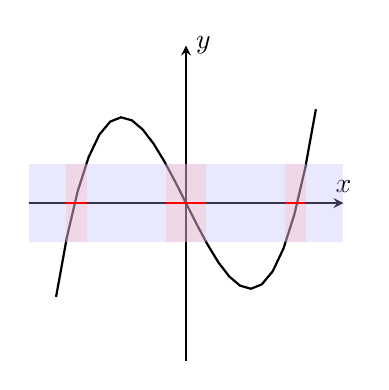
\begin{tikzpicture}[scale=1]
     \draw[->,>=stealth,semithick](-2,0)--(2,0)node[above]{$x$};%x軸
     \draw[->,>=stealth,semithick](0,-2)--(0,2)node[right]{$y$};%y軸
     \draw[thick,domain=-1.65:1.65] plot(\x,{pow(\x,3)-2*\x});

     \fill[color=blue!30, opacity=0.3] (-2,.5) rectangle (2,-.5);
     \fill[color=red!30, opacity=0.3] (-1.52,.5) rectangle (-1.26,-.5);
     \draw[thick, color=red] (-1.52,0)--(-1.26,0);
     \fill[color=red!30, opacity=0.3] (-.25,.5) rectangle (.25,-.5);
     \draw[thick, color=red] (-.26,0)--(.25,0);
     \fill[color=red!30, opacity=0.3] (1.26,.5) rectangle (1.52,-.5);
     \draw[thick, color=red] (1.26,0)--(1.52,0);
    \end{tikzpicture} 
  \end{minipage}
  \begin{minipage}[b]{0.45\linewidth}
   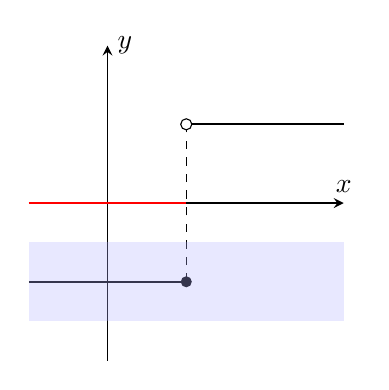
\begin{tikzpicture}[scale=1]
    \draw[->,>=stealth,semithick](-1,0)--(3,0)node[above]{$x$};%x軸
    \draw[->,>=stealth,semithick](0,-2)--(0,2)node[right]{$y$};%y軸
    \draw[thick,domain=-1:1] plot(\x,-1);
    \draw[thick,domain=1.06:3] plot(\x,1);
    \draw(1,1) circle [thick, radius=2pt];
    \fill(1,-1) circle [radius=2pt];
    \draw[dashed] (1,-1)--(1,0.94);

    \fill[color=blue!30, opacity=0.3] (-1,-.5) rectangle (3,-1.5);
    \draw[thick,color=red] (-1,0)--(1,0);
 
   \end{tikzpicture} 
  \end{minipage}
 \caption{連続関数と非連続関数}
 \label{fig:realcontinuous}
\end{figure}

一方で,次のような関数を考える.
\[
g(x) = \left\{
\begin{array}{ll}
1 & (x > 1)\\
-1 & (x \leq 1)
\end{array}
\right. 
\]
ここで$-1$を含み$1$を含まないような$Y$の開区間(例えば$(-2, 0)$)を適当にとると,この逆像は$g^{-1}((-2, 0)) = (-\infty, 1]$という区間となり,$X$の開区間にはならない.
よって関数$g$は連続ではない.実際,それは$x=1$で$y=-1$から$y=1$にジャンプしていることが図\ref{fig:realcontinuous}右からもわかる.


% 我々は2章で,4次元主義における個体を,各時間$t \in T$に対し3次元空間の部分集合$I(t) \subset \bbR^3$を割り当てる関数$I:T \to \mcalP(\bbR^3)$としてモデル化した.
% しかしこれだと,空間的に全く離れた部分や,時間の遷移に応じて「ぶつ切り」になる(たとえば特定時間$t_0$までは私で,それ以降は突然あなたというような)ものも個体に含まれてしまう.
% これがおかしいのは,通常,個体というものはその空間的・時間的部分が「繋がっている」ものだと考えられるからだ.
% これを表すために,弧状連結という概念を導入する.

連続写像を用いると,空間の部分が「繋がっている」という直観を正確に定式化できるようになる.

\begin{dfn}{弧状連結}{pathconnected}
  $(T,\mcalO)$を位相空間とする.部分集合$C \subset T$が\emph{弧状連結}(pathconnected)であるとは,任意の2点$a, b \in C$に対して,連続写像$\phi: [0,1] \to C$で$\phi(0)=a, \phi(1)=b$となるものが存在することをいう.
\end{dfn}

つまり弧状連結である部分集合は,以下の図左のように全体が「地続き」であり,任意の点から他の点までスムーズに移動できる.
一方,右図のように飛び飛びになっている集合は弧状連結ではない.
\begin{figure}[htbp]
 \begin{center}
  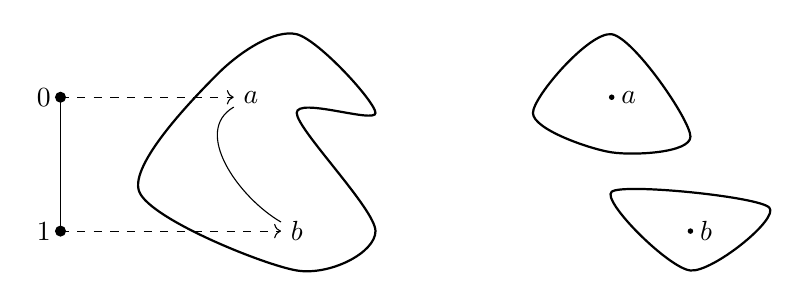
\begin{tikzpicture}
   \begin{scope}
   \draw[thick] plot[smooth cycle] coordinates{(0,0) (1,1.5) (2,2)(3, 1)(2,1)(3,-.5)(2,-1)};
   \node[right] (b) at (1.8, -.5) {$b$};
   \node[right] (a) at (1.2, 1.2) {$a$};
   \draw (a) to [out=210,in=150] (b);

   \fill(-1,-.5) circle [radius=2pt];
   \fill(-1,1.2) circle [radius=2pt];
   \draw(-1,-.5)--(-1,1.2);
   \node[left] (1) at (-1,-.5) {1};
   \node[left] (0) at (-1,1.2) {0};

   \draw[->, dashed] (0) to (a);
   \draw[->, dashed] (1) to (b);    
   \end{scope}
   \begin{scope}[xshift=5cm]
   \draw[thick] plot[smooth cycle] coordinates{(0,1) (1,2) (2,.7)(1, .5)};
   \draw[thick] plot[smooth cycle] coordinates{(1,0) (3,-.2) (2,-1)};    
   \fill(1,1.2) circle [radius=1pt];
   \fill(2,-.5) circle [radius=1pt];
   \node[right] at (1,1.2) {$a$};
   \node[right] at (2,-.5) {$b$};
   \end{scope}
  \end{tikzpicture}
 \end{center}
\end{figure}

\begin{rei}{概念の孤状連結性}{color_concept}
我々は事例\ref{rei:concept_topology}で,性質を位相空間としてモデル化した.
しかし開集合は合併で閉じているので,例えば「赤」と「緑」という性質を認めるとすると,「赤もしくは緑」という色性質も認めなければならないことになる.
これは,我々が個別に名付ける「色」は連続的に似通ったものでなければならない,という直観に反するかもしれない.
これを防ぐためには,例えば色相環のような位相空間を考え,色の性質をそのうちの弧状連結な部分集合として定義すればよい.
 \begin{center}
 \begin{tikzpicture}
 \ColourTransitionCircle[inner=1.5, outer=1.6]{yellow,red,blue,green}
 \end{tikzpicture}
 \end{center}
ここから,概念を位相的な性質によって定めるというアイデアが得られる.例えば\cite{Mormann1993-fd, Gardenfors2004-vz}などを参照.
\end{rei}

% 問題:弧状連結性が同値類を形成すること

\section{同相写像}
2つの位相空間$X, Y$は,両者が集合として異なれば別物である.
しかしそれでも,例えば半径の異なる複数の円のように,位相構造としては同一視したい場合がある.
こうした同一視を可能にするのが,\emph{同相写像}(homeomorphism)である.


\begin{dfn}{同相写像}{isomorphism}
  $(X, \mcalO_X), (Y, \mcalO_Y)$をそれぞれ位相空間としたとき,$f:X \to Y$が可逆であり,$f$もその逆写像$f^{-1}:Y \to X$も連続であるとき,$f$は同相写像であるという.
  またそのとき$X$と$Y$は\emph{同相}(homeomorphic)であるという.
\end{dfn}

つまり同相写像とは両方向に連続な全単射写像である.
両方向に連続ということは,$f$で$X$の開集合を$Y$に飛ばしても$f^{-1}$で$Y$の開集合は$X$に飛ばしても,それらの像がちゃんと開集合になっている,ということである.

たとえ$X, Y$が集合として異なっていても,両者の間に同相写像があるとき,両者は位相空間としては同じものだと理解される.
というのも,位相構造を定めるのは開集合族であるが,同相写像は2つの集合の間でこれが正確に一致している,ということを保証するからだ.
したがって,同相写像があれば,2つの位相空間は実質的には同じものとして同一視して良い.
逆に,集合としては同等だが位相空間としては異なるものもある.
2章で我々は,2つの集合間に全単射写像があるとき,それらは同等である(同じ濃度を持つ)と定義した.
同等性は集合の「集合としての」同じさを定義する.
この意味では,例えば実直線$\bbR$と実平面$\bbR^2$の間には一対一の対応があるので,集合としては同等である.
しかし$\bbR^2$から$\bbR$への連続写像は存在しないので,両者の間には同相写像がなく,よって両者は「位相空間としては」同じではない.
このように,2つの数学的構造の同じさを考える際には,どのような構造としての同じさが考えられているのかに注意を向ける必要がある.
そして位相構造の場合,同一性は同相として理解されることになる.


\begin{hatten}{}{}
2つの位相空間はどんなときに同相になるか,というのは位相幾何学の中心的な関心である.
一般の空間中の図形では,同相性は図形にあいた「穴の数」によって決まることが知られている.
つまり,元となる図形を,穴を開けたり塞いだりしないように連続的に変化させてもう一つの図形に変形することができたら,両者は同相である.
ここから,トポロジストにとってドーナツとマグカップは同じようなものだ,などと言われたりもする.
\end{hatten}


\section{分離性}
我々は4節「さまざまな位相」で,密着位相と離散位相を両極として,細かさの異なる複数の位相があることを学んだ.
開集合を集合上の点のグルーピングとすると,位相の細かさは,個々の点をどれだけ細かく分けることができるか,ということに関係している.
実際,位相空間上の任意の異なる2点をとったとき,それらを区分する開集合があるかどうか,ということは位相空間の重要な性質であり,そうした条件は\emph{分離公理}と呼ばれている.
分離公理には複数あり,それぞれが位相空間の性質を定めているが,ここではそのうち2つを取り上げよう.

\begin{dfn}{分離公理}{separation}
位相空間$(X, \mcalO)$において,次の条件を考える:
\begin{description}
 \item[($T_0$)] 任意の異なる点$x, y$に対し,どちらかのみを含む開集合($x \in O, y \not\in O$あるいは$y \in O, x \not\in O$)が存在する.
 \item[($T_1$)] 任意の異なる点$x, y$に対し,片方ずつのみを含む開集合($x \in O_x, y \not\in O_x$および$y \in O_y, x \not\in O_y$)が存在する.
 \item[($T_2$)] 任意の異なる点$x, y$に対し,片方ずつのみを含み互いに素であるような開集合($O_x \cap O_y = \emptyset$)が存在する.
\end{description} 
特に位相空間が$(T_1)$を満たすとき\emph{フレシェ(Frechet)空間},$(T_2)$を満たすとき\emph{ハウスドルフ(Hausdorff)空間}と呼ばれる.
\end{dfn}

任意の開集合$O$は集合$X$上の「似た者」グループを表す,というイメージに沿ってそれぞれを解釈すると,
$(T_0)$では全ての点のペアについて,一方のみを含み他方を含まないという意味で両者を区分するグルーピングが存在する,ということをいっている.
フレシェ性$(T_1)$はさらに進んで,全ての点が別々にグルーピングできるということをいっている($T_0$では必ずしも両方が何らかのグループに入れられている必要性はない).
一方ハウスドルフ性$(T_2)$はそれよりもさらに強く,任意の点のペアについて,被らない仕方でグルーピング可能である,ということを要請する.

\begin{rei}{不可識別者同一の原理}{PII}
ライプニッツの\emph{不可識別者同一の原理}(the principle of the identity of indiscernibles; PII)によれば,2つのモノが全く同じ性質をもつとき,両者は同一である.つまり
\[
 \forall x, y \forall F ((Fx  \Leftrightarrow Fy) \Rightarrow x=y)
\]
ただしここで$F$は任意の一項述語を表す.
事例2.2に倣って開集合を性質の外延と考えると,これは性質の空間が$T_0$だという主張だと解釈できる.
というのも,PIIの対偶を取れば,$x\neq y$ならある性質$O_F$があって,$x \in O_F$と$y \in O_F$が同値になることがない,つまり$x \in O_F \wedge y \not\in O_F$であるか$y \in O_F \wedge x \not\in O_F$であるかのどちらかということになるが,これはまさに$(T_0)$の要件と同じだからだ.
つまりPIIとは,性質空間の位相構造についての主張だと解釈できるのである\citep{Mormann2020-ly}.
\end{rei}

\begin{renshu}{}{}
同様に$(T_1), (T_2)$も,性質空間の特徴と考えられた場合,それぞれ何らかの同一性原理を主張していると解釈できる.
それらの間には$(T_2) \Rightarrow (T_1) \Rightarrow (T_0)$という含意関係があるので,対応する同一性原理にも強弱の違いがあるはずだ(例えば$(T_1)$に対応する同一性原理では,PIIよりも多くのものが同一とみなされうる).
それぞれの同一性基準がどのようなものか,考えてみよ.
\end{renshu}

\begin{renshu}{}{PII}
離散空間では,PIIはトリビアルに成立することを示せ(ヒント:離散空間で各点を区別する開集合としてどのようなものがありえるだろうか).
\end{renshu}

\begin{rei}{このもの性}{Haecceity}
Max \cite{Black1952-dz}は次のような思考実験を提示した.
二つの全く同じ性質をもった鉄球しかないような宇宙を想像してみよ.
二つの鉄球は全く同じ純鉄でできており,サイズや温度などもすべて等しい.そしてそれらは全宇宙のモノ(つまりその二つの鉄球)と完全に対称的に関係しているので,それらを区別するいかなる内的・外的性質もないことになる.
しかしこれらは依然として二つの異なる鉄球であろう------.

上の事例\ref{rei:PII}で述べたことに従えば,これはこの宇宙では$T_0$は成立しておらず,ライプニッツの不可識別者同一原理(PII)は形而上学的法則ではないという主張である.
この反例からPIIを救う一番手っ取り早い方法は,個々の事物(この場合は二つの鉄球)には,それをまさにその個物たらしめているような性質,すなわち中世哲学者が\emph{このもの性}(haecceitas/haecceity)と呼んだような性質が内属している,と考えることだ(ちなみにこの用語はラテン語で「これ」を意味する \emph{haec} に由来している).
これは位相的には,任意の事物$x$について,その事物のみが含まれる開集合$\{x\}$が存在する,という主張に翻訳できる.
そのような位相は必然的に離散位相になり,離散位相はハウスドルフ性を含意するためPIIが成立する(練習問題\ref{renshu:PII}).

しかし一方で,離散位相はあらゆる集合が「性質」として成立してしまう面白くない空間である(5節).
実際,ハウスドルフ性はかならずしも離散性を含意しない.
とすれば,このもの性というようなものを導入せずにBlackの反例に対処することも可能かもしれない.
\end{rei}

\begin{hatten}{}{}
ここではあまり触れなかったが,これらの分離性のうちハウスドルフ性は特に色々な場面で重要である.
例えば本講では扱わないが,物理学における時空間のモデルとなる多様体(manifold)では,空間がハウスドルフ性を満たすことが要請される.
\end{hatten}







\bibliographystyle{apalike}
\bibliography{m4p}


\end{document}